%!TEX root = index.tex
\chapter[Introdução]{Introdução}
\label{chap:introducao}
\section{Contextualização do trabalho}
\label{cha:contexto}

Neste capítulo será mostrado o contexto que a empresa, chamada de BC, na qual o autor realizou o trabalho de conclusão de curso estava inserida.

A empresa BeeConnect (BC), faz parte de um grupo de tecnologia chamado TM. A história da holding Techmob (TM) começa no ano de 2010 no qual um aluno da Engenharia de Produção da Escola Politécnica da USP criou uma empresa chamada Best Cool and Fun Games (BCFG). Tal empresa criou diversos aplicativos de sucesso tais como Bunny Shooter e Ant Smasher, este último atingiu recentemente mais 150 milhões de downloads na loja de aplicativos da Google. 

\begin{figure}[H]
\caption{Ant Smasher na loja de aplicativos para o sistema operacional Android}
\centerline{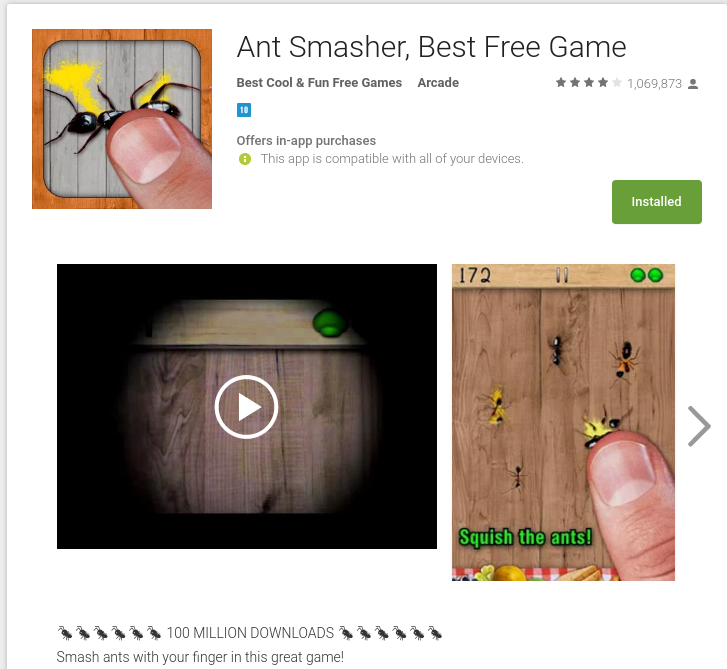
\includegraphics[scale=0.5]{img/antsmasherGooglePlay}}
\label{fig:antsmasherGooglePlay}
\caption* {Fonte: Google Play}
\end{figure}

Grande parte do fluxo de receita da BCFG vinha através de propagandas nos jogos.
\begin{figure}[H]
\caption{Banner de propaganda no Ant Smasher para iOS}
\centerline{
\includegraphics[scale=0.5]{img/antsmasheriOS}}
\label{fig:antsmasheriOS}
\caption* {Fonte: Website Revmob}
\end{figure}

Na época haviam poucas redes de propaganda que proviam um serviço de baixa qualidade para os desenvolvedores de aplicativos. Sabiamente, o fundador da BCFG resolveu criar sua própria rede de propagandas, para tirar proveito desse mercado. Surgiu então em 2011 a Revmob (RM), que rapidamente se tornou a maior rede propagandas para aparelhos móveis da América Latina.

\begin{figure}[H]
\caption{Website RevMob para o Brasil}
\centerline{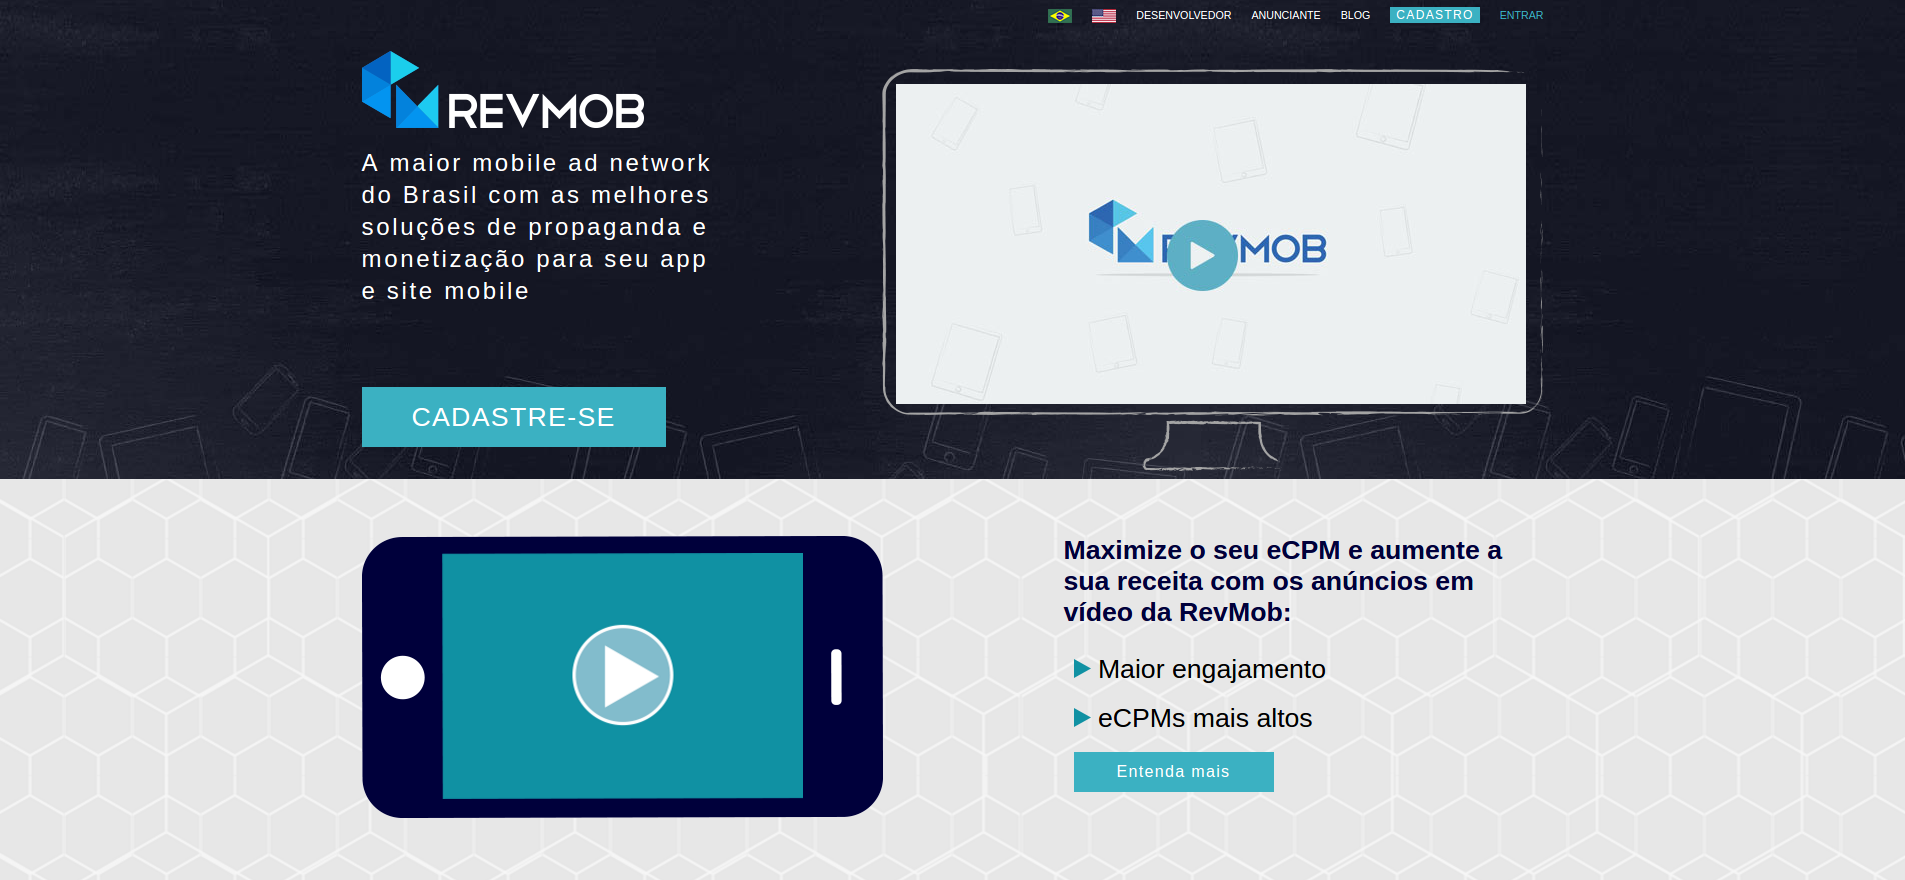
\includegraphics[scale=0.5]{img/screenshotSiteRev}}
\label{fig:screenshotSiteRev}
\caption* {Fonte: Website Revmob}
\end{figure}

O mercado de redes de anúncio cresceu rapidamente e se tornou muito competitivo. As grandes vantagens competitivas nesse mercado são:
\begin{itemize}
\item Servir rapidamente o anúncio, baixa latência, em questão de menos de 100 milissegundos.
\item Saber estimar as taxas de conversão de um anúncio. Para cada vez que o anúncio aparecer qual a chance dele ser clicado, e para cada clique qual a chance do aplicativo ser instalado.
\item Saber aumentar as taxas de conversão de uma propaganda. Geolocalização precisa e saber as informações da pessoa para o qual o anúncio está sendo mostrado aumentam bastante as taxas de conversão.
\end{itemize}

O desafio da latência foi resolvido através de uma reestruturação dos sistemas e de reescrita do código. Para endereçar o desafio da estimativa das taxas de conversão foi necessária a criação de uma nova empresa chamada Beluga, criada em 2014. As soluções de Big Data eram demasiadamente caras e de difícil integração com o sistema da Revmob. E sobre o aumento das taxas de conversão a Revmob decidiu focar na questão da geolocalização precisa, através da tecnologia de beacons, o que culminou no nascimento da empresa Beeconnect em 2015, que será o foco desse trabalho de formatura.

\section{Definição do Problema}
\label{cha:problema}
A Beeconnect surgiu para externalizar os conhecimentos obtidos com as demais empresas do grupo Techmob. A empresa nasceu com 4 pessoas com a supervisão de um membro do Board da Techmob.

A empresa queria tirar proveito da tecnologia de beacons que estava na moda em 2015, porém poucos no Brasil tinham ouvido falar. O beacon é um aparelho que utiliza a tecnologia Bluetooth Low Energy e é utilizado para geolocalização indoor com uma ótima precisão, superando em muito o GPS.
\begin{figure}[H]
\caption{Funcionamento app Beeconnect}
\centerline{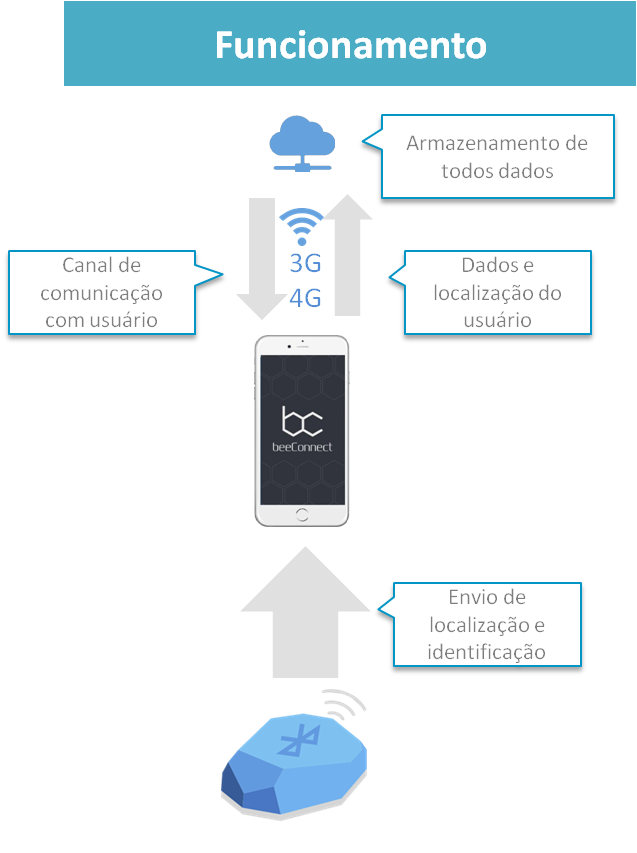
\includegraphics[scale=0.5]{img/explicacaoBeeconnect}}
\label{fig:explicacaoBeeconnect}
\caption* {Fonte: Material de marketing da Beeconnect}
\end{figure}

A equipe fez diversas análises de como os beacons estavam sendo utilizados no exterior e descobriu diversas aplicações em lugares diversos como shoppings, aeroportos, hospitais, hotéis e museus.

\begin{figure}[H]
\caption{Aplicação de beacon em shopping}
\centerline{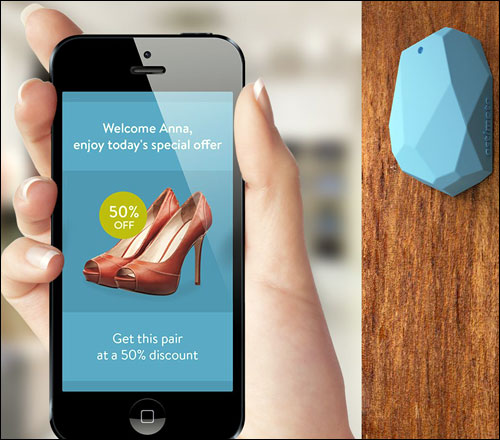
\includegraphics[scale=0.5]{img/beaconShopping}}
\label{fig:beaconShopping}
\end{figure}

\begin{figure}[H]
\caption{Aplicação de beacon em aeroporto}
\centerline{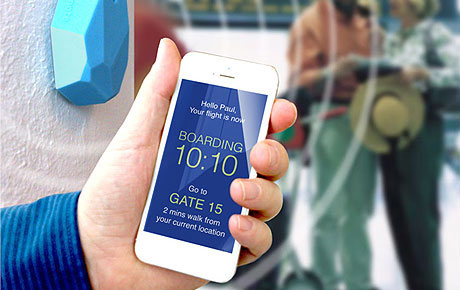
\includegraphics[scale=0.5]{img/beaconAeroporto}}
\label{fig:beaconAeroporto}
\end{figure}

\begin{figure}[H]
\caption{Aplicação de beacon em hospital}
\centerline{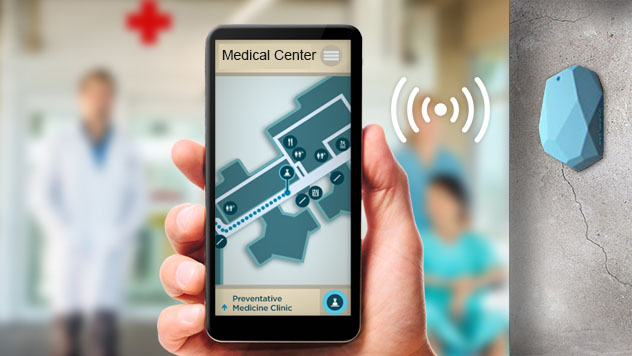
\includegraphics[scale=0.5]{img/beaconHospital}}
\label{fig:beaconHospital}
\end{figure}

\begin{figure}[H]
\caption{Aplicação de beacon em hotel}
\centerline{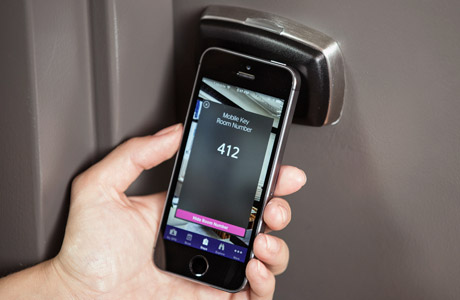
\includegraphics[scale=0.5]{img/beaconHotel}}
\label{fig:beaconHotel}
\end{figure}

\begin{figure}[H]
\caption{Aplicação de beacon em museu}
\centerline{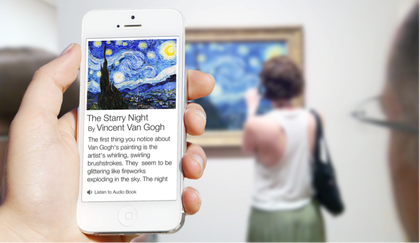
\includegraphics[scale=0.5]{img/beaconMuseu}}
\label{fig:beaconMuseu}
\end{figure}

Um dos membros da equipe utilizou um contato que trabalhava em um grande shopping da capital paulista e agendou uma reunião para apresentar a tecnologia de beacons e o valor que a Beeconnect conseguiria gerar para eles. Rapidamente a equipe desenvolveu  um produto que serviria para mandar propagandas geolocalizadas, trabalhando cerca de 16 horas por dia por uma semana, que consistia em:
\begin{itemize}
\item Um aplicativo para iOS que possuía um SDK (basicamente um software) que permitia a comunicação com beacons.
\item Um servidor que fazia a comunicação com o aplicativo e gravava todas as informações de distância do celular em relação ao beacon e enviava uma propaganda para o aplicativo.
\end{itemize}

Na apresentação para o Shopping a equipe sequer apresentou o produto desenvolvido dado o desenrolar da reunião.

Todos ficaram muito frustrados com o tempo perdido e a sensação de que haveria um jeito melhor de ter desenvolvido o projeto sem ter gasto esforços com tarefas desnecessárias ou que não tinham um valor claro a ser gerado.

A equipe então começou a vender a ideia do que o beacon poderia fazer e criar o produto junto com o cliente. Basicamente utilizou-se o processo de vender apresentações em slides para validar a ideia. Foram feitas reuniões com diversos tipos de clientes: hospitais, hotéis, construtoras, concessionárias e varejistas. Após essas reuniões o foco da empresa ficou mais claro. O varejo pareceu ser a opção mais rentável.

Após acumular alguns clientes interessados ficou evidente a necessidade da criação de um produto para ser testado. A pressão por resultados fez até o autor abrir mão da graduação na Escola Politécnica para trabalhar cerca de 14 horas por dia para liderar o desenvolvimento tanto de um servidor quanto um aplicativo para smartphones Android. Houve mais contratações para auxiliar tanto em vendas quanto no desenvolvimento.

O produto criado foi um aplicativo de descontos chamado iShop, que utilizava a tecnologia de beacons para gerar um cupom de desconto somente na loja física cadastrada. O primeiro piloto para testar esse produto foi realizado no McDonald's localizado na Riviera de São Lourenço.

Houve a geração e utilização de alguns cupons no local, entretanto nada muito relevante, a distância entre o local do piloto e o escritório na empresa deixava inviável um acompanhamento de perto.

Por motivos estratégicos a matriz do McDonald's do Brasil pediu para que o piloto fosse cancelado. Além disso, o advogado da Techmob sugeriu que o nome do aplicativo fosse mudado porque dificilmente algum nome de marca com "i" no começo seria registrado. Assim, a equipe decidiu registrar a marca Beeconnect e utilizá-la como nome do aplicativo também. Foi necessária também uma reformulação no design do aplicativo para que ficasse condizente com a marca.

Após tais insucessos a empresa conseguiu fechar um piloto com o maior varejista da América Latina, o Grupo Pão de Açúcar. Foi realizado um piloto na loja dentro da sede da empresa. A promoção foi "Todas as cervejas premium com 50\% de desconto". O resultado foi um sucesso. Vários funcionários baixaram o aplicativo na hora e conseguiram utilizar o desconto sem problemas. O resultado do piloto foi um contrato assinado no qual seriam implementados beacons em todas as lojas de formato de proximidade premium, chamadas de Minuto Pão de Açúcar, no estado de São Paulo.

Após a implementação dos beacons em todas as Minuto Pão de Açúcar, esperou-se um resultado condizente com o esforço. Infelizmente tal resultado não veio. A pressão resultados do board da Techmob veio. A holding havia gasto cerca de R\$500.000 reais até então.

\section[Objetivos]{Objetivos}
\label{chap:objetivos}

Muitos problemas da BC se deram em virtude da falta de planejamento e de não usufruir de um modelo de plano de negócio para startups. O objetivo deste Trabalho de Conclusão de Curso com o professor André Fleury foi tentar estabelecer um modelo baseado nos conceitos dos autores Eric Ries e Steven Blank para salvar a Beeconnect.